\documentclass{reading_glasses}
%\usepackage{graphicx}
%\usepackage[pdftex]{graphicx}
%\usepackage{subfig}
%\DeclareGraphicsExtensions{.pdf,.png,.jpg}



\makeatletter
\let\@copyrightspace\relax
\makeatother

\begin{document}

\title{Summary of Testing Network-based Intrusion Detection Signatures using Mutant Exploits}

\numberofauthors{1}
%
\author{
    \alignauthor
    Matthew Beldyk\\
    \affaddr{University of Colorado}\\
    \affaddr{Boulder, Colorado}\\
    \email{beldyk@colorado.edu}
}
\maketitle
\begin{abstract}
\end{abstract}

\section{Introduction}

\section{Setting}
Modern computer systems have many various ways to detect penetration attempts.  These advances have made the job of the perpetrator much more difficult, but not impossible. Vigna et al. present a methods to modify how an attack appears without losing functionality.  

There are two types of intrusion detection: network based and host based.  Network based detection relies on inspecting packets for patterns that are related to an attack.  When various attacks are discovered, researchers and developers work to find a pattern that will match these various attacks, but will not have too many false positives.  These patterns look for many different things.  For example, a no-op sled or a long sequence of ../../../ in a browser request might trigger a response.  These responses can range from alerting the administrator, to dropping the packet to blacklisting the offender’s ip address.  Host based detection looks for specific behavior on a machine that might indicate that an intrusion has taken place.  For example, these tools might notice ports being opened that wouldn’t be expected or other unexpected behavior. These patterns that help identify attacks are often called signatures.  The work to create these signatures must often be done quickly to counter attacks that are already being preformed, and therefore it is possible for holes to appear in the code logic.  Various permutations of the attack might be missed, or the patterns that are being looked for might be too restrictive.   This is a trade off that developers of these tools must make.  Should a product flag more things, but possibly interrupt non-malicious business related traffic, or should the product detect less things, but allow all normal business traffic to get through the system.  Optimally, a system should detect 100\% of the attacks and should have no false alarms, however, this is not the case in practice.

Vigna et al. present their tests about the effectiveness of two popular network intrusion detection systems: Snort and IIS RealSecure.  They present a number of test and ways to modify attacks such that the attack remains effective, however they are no longer detected via the tool in use.  
The basic context of the problem that Vigna et al. are looking at is within the context of networks protected with either Snort or IIS RealSecure .

\section{Problem}
To enter a system that has a network intrusion system presents to an interesting challenge.  First, one must simply find a way to break into the systems, secondly, one must do this without raising the alarm of the network intrusion detection systems.  The authors test their systems against two tools: Snort and RealSecure.  They also present a number of challenges that they must break once they are past the system.    The author's basic approach was to take a known exploit for a vulnerability then modify it in various ways to see if it can get past the network intrusion detection system.  In the paper, the authors present a number of ways to subtly modify an attack such that it might get past signature based detection (the authors refer to this as muting an attack.)  The authors suggest using both network layer mutations and application layer mutations.

\subsection{Network Layer Mutations}
Using IPv6 is the first network layer mutation suggested by the authors.  IPv6 is a system that has not yet been implemented nor supported by many systems yet, and the theory is that the network intrusion detection systems might not be looking for things using this new protocol and the attack could slip past.  IP packet splitting is another method suggested by the authors to evade detection.  Basically, an attack would be split between many packets instead of being in a single packet.  This works on the theory that for a network intrusion detection system would need to keep track of every packet, and track changes between packets that might arrive at very different amounts of time.  In practice, this would use way to much space and processing power to be practical.

\subsection{Application Layer Mutations}
The authors suggest quite a number of application layer mutations to possibly bypass network intrusion detection systems.  The basic idea of these it that servers are generally written to be very forgiving in terms of what they accept, far more so than the raw information in the specifications of the protocols might lead a developer to expect.  There are many ways to subtly modify what is sent to a server that, which technically invalid, will be accepted and used by the server.  The theory with these modifications is that the developers of the network intrusion detection systems will not have coded every possible "semi-valid" modification into their signatures.

The first application layer mutation suggested is Protocol Rounds.  Basically, when two systems send messages back and forth, a single connection is often reused.  For example, HTTP 1.1 will reuse the same connection (until some inactivity timeout value is reached) the client is browsing through.  Some network intrusion detection systems only look at the initial transactions through these connection channels, so one can simply send some valid responses that look like usual browsing traffic, and then switch to sending the actual attack information.  Again, checking of only the initial connection is done for performance reasons (although the authors do suggest it might also simply be a bug in the detection tool.)

The authors also suggest embedding control sequences in the middle of an otherwise valid FTP command.  The tools might detect these control sequences one their own, but might not if they are within something that otherwise looks valid.  It is also possible to use alternative control sequences to bypass the network intrusion detection systems.  

An approach suggested for HTTP is to take advantage of the inherent tolerance of an HTTP server and send slightly wrong commands.  For example, one can omit the carriage return after the newline and most HTTP servers will still respond favorably to the request.  The network intrusion detection systems are expecting valid HTTP requests and the "wrong" request might go unnoticed.  

Adding NULL records into SSL transactions is another way that signature based detection can be avoided.  Technically, null records are not allowed by the specification; however, many implementations do allow these null records.

\subsection{Exploit Layer Mutations}
It is also possible to change the actual exploit so that it no longer matches any signatures.  This must be carefully done so that the exploit still runs, but there are a number of ways to do that.  

The first method proposed is Polymorphic Shellcode.  This basically means creating shellcode that will modify itself in various ways to bypass the network intrusion detection systems.  For example, the shellcode could include an encrypted or obfuscated payload that could be decrypted when ran.  The code would need to include the code to do this decryption, but some of the simplest encryption techniques (such as XORing the shellcode with some value) might be enough to bypass the detection techniques.  Also, NOPs and other non-destructive instructions can be added randomly to the shellcode with the theory that the code will no longer match a signature.  

The other method described to avoid exploit layer detection is to use an alternative encoding of the payload.  The payload could be encoded with ZIP or TAR and depending on what software the server is running, might be automatically decoded.  It is also possible to try transmitting the exploit as BASE-64 or URL encoded as these might also not be detected.  The network intrusion detection systems might not be looking for levels of indirection as deep as something compressed before it is sent or stored in some different format.

\section{Experiments}
The authors created a framework in python to take exploits and subtly modify them and then send the exploit to the target server. \ref{fig:sploitF}  This system can also detect when an exploit has been successful.  For the purposes of the experiment, the payload would either create some file on the server in a known location and this could be detected or the payload would send some message back to the framework indicating success. The basic framework would “randomly” mutate the various attacks and payloads to attempt to get them past the two filters.  Each time the system was started, it would be started with a specific seed so that the results could be reproducible.

\begin{figure*}
	\centering
	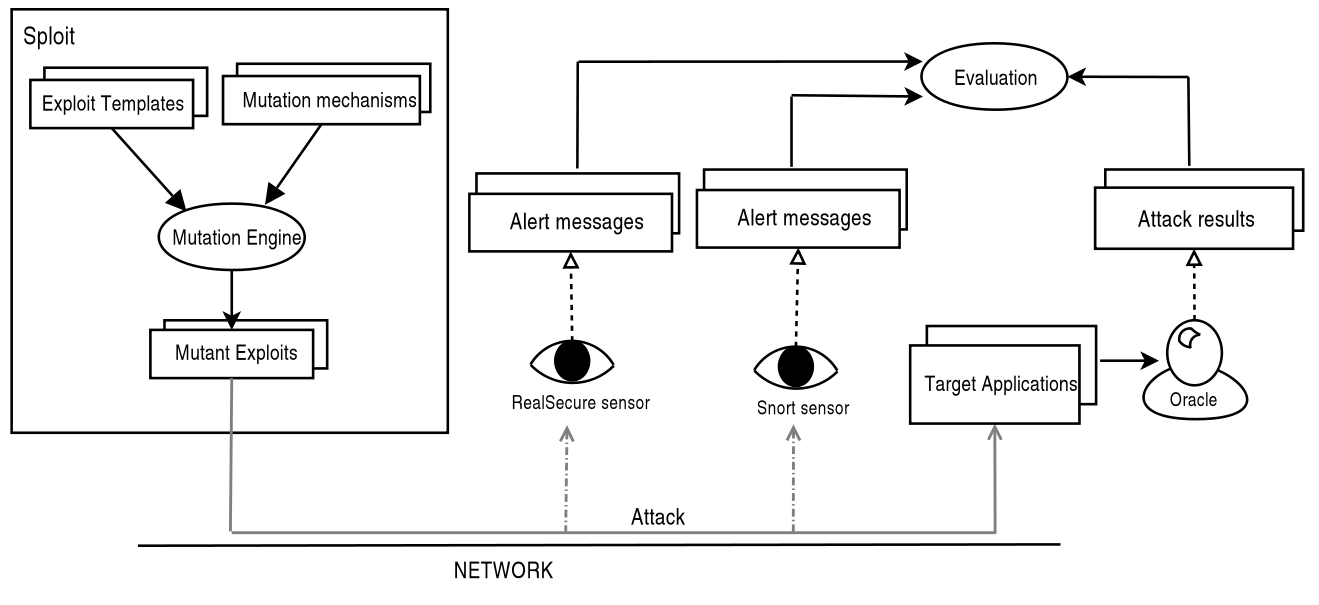
\includegraphics[width=1.0\textwidth]{SploitFramework.png}
	\caption{Sploit Framework Diagram}
	\label{fig:sploitF}
\end{figure*}

The test platform for the experiments was a Linux server running the attacking software, a second Linux server running either Snort or RealSecure, and a selection of target hosts running a number of different operating systems.  There were also a number of vulnerable applications installed on the target hosts.

The exploits were chosen explicitly to cover a great range of services and that led themselves to be easily mutable.  The authors chose a selection of exploits that worked across several operating systems and worked with a number of different protocols.  The authors also targeted several types of attacks including buffer overflow, directory traversal, and denial of service.  In the paper the authors list their various attacks as well as an overview of how each of the attacks work.

The attacks were against two common network intrusion detection systems: Snort and RealSecure.  Snort is an open source framework with a large selection of signatures and pre-processors to unwrap data from various protocols into a normalized data-model that can be compared to the signatures.  IIS’s RealSecure is a commercial network intrusion detection system; it detects attack using a set of complex closed source rules.

\section{Results}
When the authors ran their experiments they found that the two tools correctly identified all of the unmodified attacks.   Of the things that were tested, Snort fared the best with only six out of ten of the attack vectors succeeding in evasion; \ref{fig:snortRes} RealSecure fared worse with nine out of the ten succeeding. \ref{fig:realSecRes}  The authors note that one should not draw conclusions about the quality of the tools from these raw numbers due to them not searching the entire attack space and the system stopping attacking a particular vulnerability once an attack that had succeeded was detected.  As an interesting note, the results of what succeeded appear to indicate that the easiest way to bypass RealSecure is to prepend carriage returns into the attack.   Also the authors noted how easy it was to bypass either of these tools using automated attack mutation tools.  

%\figure{put pictures here}
\begin{figure*}
	\centering
	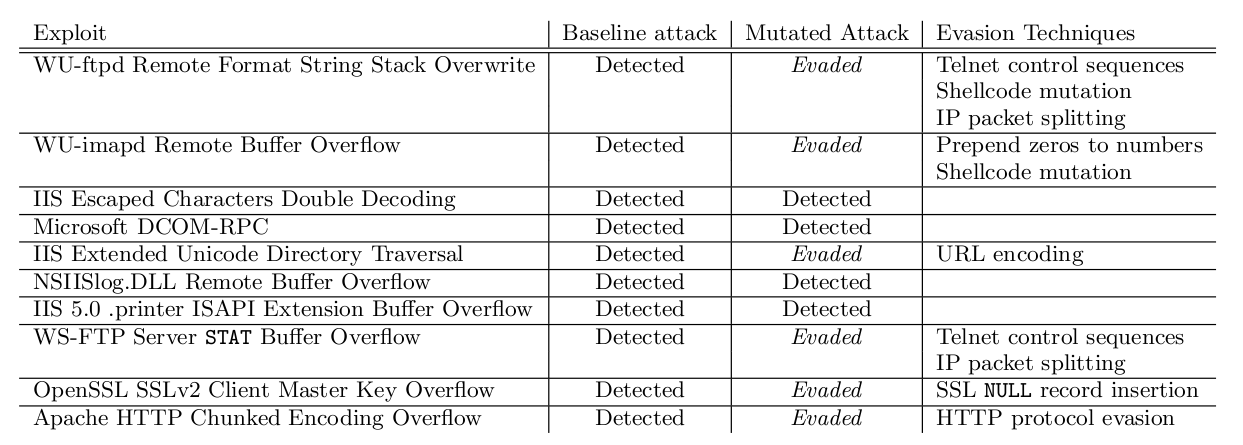
\includegraphics[width=1.0\textwidth]{SnortResults.png}
	\caption{Evaluation Results for Snort}
	\label{fig:snortRes}
\end{figure*}

\begin{figure*}
	\centering
	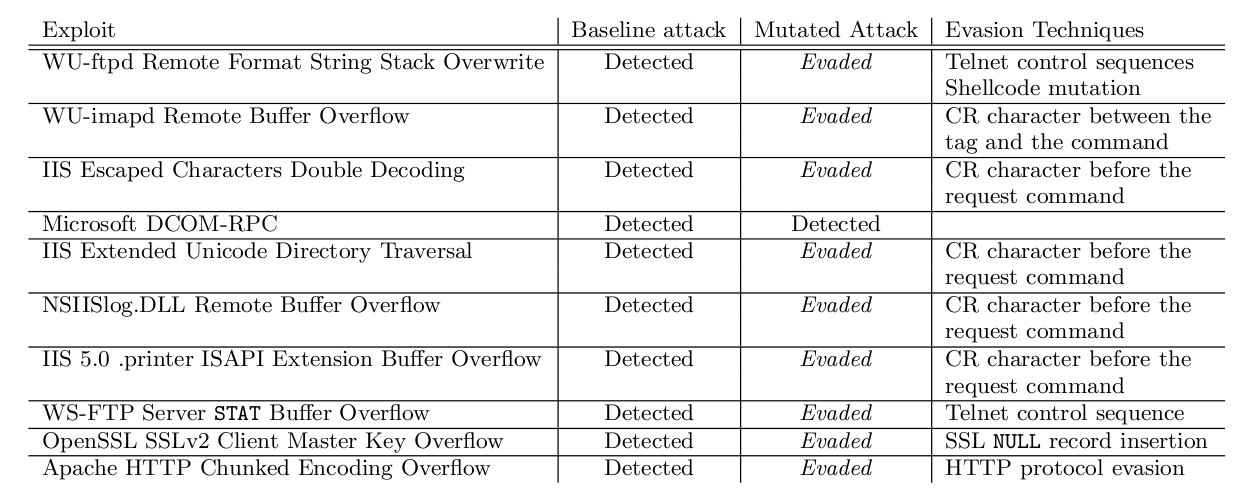
\includegraphics[width=1.0\textwidth]{IISRealSecureResults.png}
	\caption{Evaluation Results for Snort}
	\label{fig:realSecRes}
\end{figure*}

\section{Implications}
This paper calls into question the effectiveness of signature based network intrusion detection systems.  Writing signatures to detect all possible attacks is a time consuming and difficult, if not impossible, task.  When an attack is detected developers of these tools must react quickly to push out a new signature that may not have had a chance to become completely airtight, and thus errors and holes are introduced into these products.  

The immediate impact of this paper are for hackers to create tools that automatically obfuscate attacks in novel ways.  An immediate problem would be to test an obfuscated attack on a target network, and discover that indeed these tools do detect that particular obfuscation and alert the sysadmin that something interesting is happening.  This can be countered by downloading the newest version of this software and testing the attack locally with a similar framework to mutate and obfuscate the attack to find some permutations that are not detected.  

Another thing that I can see happening as a result of this paper is for companies to have multiple network intrusion detection systems.  Since these two tools had different holes in their detections, it would make logical sense that having the two in tandem would close both of those holes.  An obvious issue with this is the creation of more false positives.  I can speak from personal experience that being on the wrong end of false positives for malicious network behavior can be incredibly frustrating.  In undergrad, there was a system that detected spurious packets on the network and would turn off access to a physical port for a single packet of strange traffic; this made it nearly impossible to do homework when whenever I sent out of band reset packets (which apparently matched the signature of a virus.) my network was turned off.

Although the immediate impression of this paper is that it will weaken the effectiveness of these signature based network intrusion detection tools, this may not be the case.  If the developers of these tools were to use a similar framework to test their signatures and predictable mutations, this would illustrate a number of possible bugs that could be cleaned up before deployment of a new signature.  They could do a sort of fuzzing unit testing to make sure that the logic works properly and only allows through valid traffic and flags the bad.  In general, automated testing often leads to improved code quality.

\section{Questions}
There are a number of questions that arise after reading this paper.  How do these results apply to virus detection via regular virus checkers?  Are there similar results and viruses that mutate and change their signature will become beyond detection?  I know for a few years, all people seemed to complain about was getting viruses on their computers, but I hear a lot less of that now.  For virus detection there is the added issue of having to remove the virus from the system and if the virus had behavior that would cause it to hide in different places on the infected machine this would make that challenge even more onerous.  

An obvious omission in this paper is the issue of false positives.  The authors only discuss this from the point of view of the attacker who just needs to get an attack through the system without detection.  An important quality of these systems is to have a low number of false positives.  If these systems have too many false positives, they will suddenly be inflicting their own denial of service attack on the systems they are supposed to protect from such a thing.  However, these false positives might be less of an issue than one might expect.  A malformed request is still a malformed request, and it might make sense to drop this request whether or not it is an attack or not.  It would really have to depend on the context of the malformed request.


\bibliographystyle{abbrv}
\bibliography{nids_evasion}

\end{document}

